\section{Uniform endpoint-free laws and moments}\label{R:cal:uniform-section}
The absolute estimates of Section~\ref{R:cal:geometry-section} give upper
spatial tails under every law considered here. The remaining issue for a
uniform endpoint-free walk is a lower bound on its endpoint displacement.
In the half-plane we compare nearby lengths by adjoining a long initial
bridge. In the plane we insert that bridge at a minimum and count the
possible inverses. Both comparisons yield a lower law on a common set of
lengths of natural density one. We first record the moment consequences
of the absolute upper bound. For a walk $\gamma$ started at $\gamma_0$,
its maximum radius is $\max_j|\gamma_j-\gamma_0|$; it lies between
half the diameter and the diameter.

\subsection{Upper tails, moments, and the half-plane comparison}
\label{R:cal:consequences}
\begin{theorem}[Moment and half-plane consequences]\label{R:cal:halfplane-laws}
For the independent-irreducible infinite walk, and for uniform strict
bridges at every sufficiently large even center length $n$, both endpoint
distance and maximum radius have positive-moment powers $3p/4$: for either
variable $R_n$,
\[
 \mathbb E R_n^p=n^{3p/4+o(1)}\qquad(p>0\text{ fixed}).
\]
The same holds for the vertex-bridge conventions of
Section~\ref{R:cal:section}.

For endpoint-free uniform walks in the plane or half-plane, the probability
of maximum radius exceeding $n^{3/4+\epsilon}$ is smaller than every fixed
inverse power of $n$, for each fixed $\epsilon>0$. In the half-plane there
is one natural-density-one set of lengths along which endpoint distance and
maximum radius have exponent $3/4$ in probability and all the preceding
positive-moment exponents.

Under the half-plane law of free center length $n\ge1$ with weights
$\rho^n e^{-tn}$, length is $t^{-1+o(1)}$ and endpoint distance and maximum
radius are $t^{-3/4+o(1)}$ in probability as $t\downarrow0$; their positive
moments have the corresponding powers. At fixed bridge height $h$, the
critical bridge length is $h^{4/3+o(1)}$ both in probability and in first
mean.
\end{theorem}
\begin{proof}
\textit{Absolute upper tails and moment bounds.}
For the infinite walk, consider the first $n$ whole irreducibles; their
concatenation contains the first $n$ centers. Except with probability
$Cn^{1-aA}$, every one of these pieces has diameter at most $n^A$, where
$A$ is any sufficiently large fixed constant. The concatenation has
exactly its critical bridge weight as probability, by unique
factorization. Split it at its $n$th center. If this prefix reaches radius
$n^{1/d_*+\epsilon}$, summing its critical mass over diameter dyads costs
stretched-exponentially little by \eqref{R:cal:fast-mass}, with its slack
$\xi$ sufficiently small. The remaining suffix has diameter at most
$Cn^{A+1}$ and costs at most $CV_{Cn^{A+1}}$, including bounded endpoint
weight corrections. Choose the exponent $\nu$ in
\eqref{R:cal:volume-bound} sufficiently small after $A$; this suffix factor
is absorbed by the stretched-exponential bound. Since $A$ can be
arbitrarily large, the upper tail for the first $n$ centers is smaller
than every fixed inverse power of $n$.

The almost-sure lower exponent of Theorem~\ref{R:renew:infinite}, this
upper tail, and the deterministic linear distance bound give the stated
moments for endpoint distance and maximum radius. For uniform strict or
vertex bridges, divide the absolute fast-path bound by their previously
proved polynomial lower mass bound and use their typical lower cutoff.
The same argument gives the upper tail for uniform endpoint-free walks.
For plane walks the total edge-weighted mass is at least one, by the
connective constant and submultiplicativity. For half-plane walks it has
a polynomial lower bound by inclusion of strict bridges, with one outward
center appended when required by parity.

\paragraph{Long prefixes compare nearby half-plane lengths.}
Let $h_n$ be the total $\rho^n$-mass of the $n$-center half-plane paths
rooted at the prescribed inward center. Fix a small $\epsilon>0$ and a
dyad $N\le n<2N$. Put
\[
 k=\lfloor N^{\alpha-2\xi}\rfloor,\qquad
 L_0=\lfloor N^{1-\xi}\rfloor,\qquad \alpha=9/16,
\]
with $0<\xi<3\epsilon/16$. Call a tuple of the first $k$ independent
irreducibles good when its total length $l$ is at most $L_0$ and its
height exceeds $N^{3/4-\epsilon/2}$. Its probability $w_N$ tends to one:
the length failure is at most $Ckq_L(1/L_0)=o(1)$, and height damping
bounds the other failure by
$\exp\{1-cN^{3\epsilon/8-2\xi}\}$.

Adjoin to each good tuple an arbitrary nonempty half-plane continuation
above its final port. These events are disjoint for different tuples,
as in Theorem~\ref{R:renew:uniform}. Their combined probability in the
uniform length-$n$ law is therefore
\[
 p_n=w_N\,\mathbb E_{\rm good}[h_{n-l}/h_n]\le1.
\]
The distribution of $l$ in this expectation depends on $N$, not on $n$.
The volume upper bound and bridge lower bound give
$|\log h_j|\le C_\nu N^\nu$ throughout $N-L_0\le j\le2N$, for each
fixed $\nu>0$. Jensen's inequality and $1-p_n\le-\log p_n$ yield
\[
 \sum_{N\le n<2N}(1-p_n)
 \le -N\log w_N+
 \mathbb E_{\rm good}\sum_{N\le n<2N}(\log h_n-\log h_{n-l}).
\]
For each fixed shift $l$, the interior terms cancel. The remaining two
boundary intervals have total length at most $2L_0$, so their contribution
is $O_\nu(N^{1-\xi+\nu})=o(N)$ when $\nu<\xi$. Thus the average failure
probability tends to zero. On a good-tuple event, the endpoint stays above
the final tuple height and hence has distance at least
$n^{3/4-\epsilon}$ for large $N$.

Together with the all-length upper tail, this proves the claimed lower
and upper cutoffs outside a vanishing fraction of each dyad. Choose
exponent slacks and probability-error thresholds tending to zero
sufficiently slowly over successive dyads. The retained lengths form
one natural-density-one set on which the probability conclusion holds.
On this same set the lower cutoff and the superpolynomial upper tail,
with the linear deterministic bound, give every fixed positive moment.

\paragraph{Half-plane thermal and fixed-height consequences.}
For the half-plane Boltzmann law take $N=\lceil1/t\rceil$ and the same
good tuples. The suffix partition is exactly the original half-plane
partition, so the good-prefix probability is
$w_N\mathbb E_{\rm good}e^{-tl}\to1$. The volume bound makes lengths
larger than $N^{1+\delta}$ superpolynomially unlikely, even after
multiplication by any fixed length power. Below this cutoff, condition
on length and apply the uniform upper spatial tail. Lengths below
$N^{1/2}$ cannot violate the spatial upper cutoff by the linear bound,
and the good-prefix lower cutoff makes them atypical. Taking $\delta$
and the speed slack sufficiently small proves the spatial upper bound
and all positive spatial moments. The endpoint lower bound combined
with the speed bound also rules out every length lower power
$N^{1-\delta}$, giving the length statement and its moments.

At a fixed bridge height $h$, the short-length tail is negligible by
\eqref{R:cal:fast-mass}, since the diameter is at least a constant times
$h$ and the denominator is $B_h\asymp h^{-\vartheta}$. To bound the mean,
first restrict diameter to $r=Ch\log h$. The finite chord bound
\eqref{R:cal:box-moment}, applied in a common convex box to order-$r$
translates of the fixed source, bounds the first-length mass by
$r^{13/12+o(1)}$. For larger diameters, the exponential strip cutoff
and the deterministic area bound make the length-weighted tail
negligible when $C$ is large. Division by $B_h$ gives mean length at
most $h^{4/3+o(1)}$ and hence the typical upper cutoff; the short tail
gives the matching lower bound for the mean.

The same length-versus-scale conclusion holds for arches from a fixed
half-plane source with terminal gap in $[h,2h]$ on one side and diameter
at most $Ch$, for sufficiently large fixed $C$. The confined pointwise
arch lower bound gives denominator at least $ch^{-\vartheta}$, and the
same translated first-moment and fast-path estimates apply.
\end{proof}

\subsection{Unrestricted walks by insertion at a minimum}\label{R:cal:refolding}
A full-plane walk need not begin with a long bridge. We create one by
reflecting the part before a minimum and separating it from the part
after that minimum. An output can admit many such insertions in reverse.
We first bound this multiplicity, then compare masses at nearby lengths.

\begin{theorem}[Unrestricted spatial laws by refolding]\label{R:cal:plane-laws}
For full-plane uniform walks rooted at a fixed center, there is a set
$\mathcal N\subset\mathbb N$ of natural density one such that, as
$n\to\infty$ through $\mathcal N$, endpoint distance and maximum radius
are $n^{3/4+o(1)}$ in probability. For every fixed $p>0$ their $p$th
moments are $n^{3p/4+o(1)}$ on the same set.
Under the normalized full-plane law with edge weights $(\rho e^{-t})^n$,
as $t\downarrow0$ the length is $t^{-1+o(1)}$ and both spatial variables
are $t^{-3/4+o(1)}$ in probability, with corresponding positive-moment
powers. The thermal assertion holds without exceptions in $t$.
\end{theorem}

Write $c_m$ for the total critical mass $\sum\rho^m$ of $m$-edge walks
from a fixed center. Lattice symmetry identifies the two starting center
types. We have $c_m\ge1$ and, by \eqref{R:cal:volume-bound},
\[
 0\le\log c_m\le C_\nu(1+m)^\nu\qquad(\nu>0).
\]
Throughout this argument $d_*=4/3$, $a=3/4$, and $\vartheta=1-a$.

\paragraph{The insertion and its inverse.}
Fix one lattice normal. Walks whose endpoints realize its two global
height extrema, in either order, have total critical mass $o(1)$ at
length $m\to\infty$. Indeed their bounded endpoint extensions are strict
port bridges. Their exact-length masses $u_l$ tend to zero: each fixed
piece-count term tends to zero, and the remaining terms are dominated
by the summable envelope $k^{-1/\alpha+o(1)}$ from
\eqref{R:cal:length-atom}. Call the walks not omitted eligible.

Write $a_0,b_0$ for the input endpoints. Choose an internal global height
extremum of each eligible walk by a fixed deterministic rule. Choose the sign of the normal coordinate $y$
so it is a minimum $v$; the two signs will be counted separately. The
two used edges at $v$ are the rising slants. Let $P$ be the wall just
below $v$, with its port adjacent to $v$. All input vertices lie
strictly above $P$. Reflect the incoming arm, including $v$, across
$P$, insert a strict upward bridge from that port to a port on a wall
$Q$, and translate the outgoing arm, including $v$, by the bridge's
port increment. The three parts lie in disjoint open slabs and form a
self-avoiding walk. Translate it once more to a fixed output center of
the type produced by reflection; its mass $c_n$ agrees with the other
starting type by lattice symmetry.

Use bridges of center length $l$ satisfying
\[
 s\le Q-P\le2s,\qquad l\le C_0s^{d_*}.
\]
The resulting edge length is $n=m+l+1$: the minimum center has been
duplicated. Its weight is the input weight times $\rho^{l+1}$. Let
$A_l$ be the total critical mass of the allowed inserted bridges of
length $l$, and put $A=\sum_l A_l$. These masses do not depend on the
input. Proposition~\ref{R:cal:inputs} gives confined bridge mass
$\asymp s^{-\vartheta}$ and first-length mass at most $Cs^{13/12}$
at each height in the bin. Thus, for sufficiently large fixed $C_0$,
\[
 A\asymp s^a.
\]
Figure~\ref{R:cal:refolding-figure} shows the construction before the
common translation that fixes the output root.

\begin{figure}[ht]
\centering
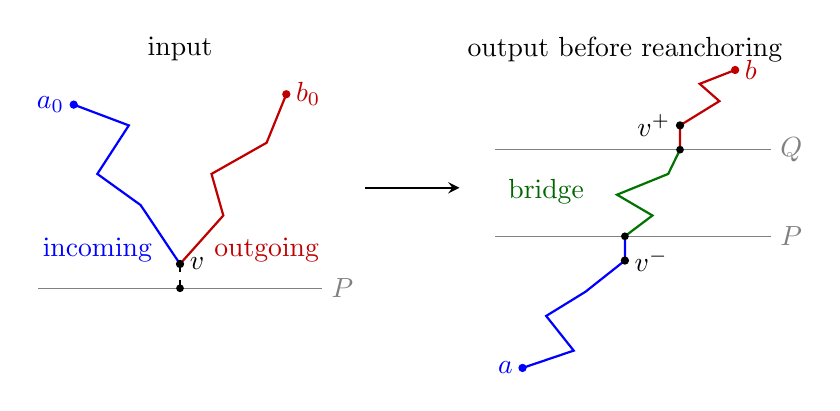
\begin{tikzpicture}[x=1cm,y=.88cm,>=stealth]
 \begin{scope}[xshift=-3.4cm]
  \node at (0,3.45) {input};
  \draw[gray] (-1.8,0)--(1.8,0) node[right] {$P$};
  \draw[thick,blue] (-1.35,2.65)--(-.65,2.35)--(-1.05,1.65)
    --(-.5,1.2)--(0,.35);
  \draw[thick,red!75!black] (0,.35)--(.55,1.05)--(.4,1.65)
    --(1.1,2.1)--(1.35,2.8);
  \draw[dashed] (0,0)--(0,.35);
  \fill (0,0) circle(1.4pt);
  \fill (0,.35) circle(1.5pt) node[right] {$v$};
  \fill[blue] (-1.35,2.65) circle(1.5pt) node[left] {$a_0$};
  \fill[red!75!black] (1.35,2.8) circle(1.5pt) node[right] {$b_0$};
  \node[blue] at (-1.05,.55) {incoming};
  \node[red!75!black] at (1.1,.55) {outgoing};
 \end{scope}
 \draw[->,thick] (-1.05,1.45)--(.15,1.45);
 \begin{scope}[xshift=2.25cm]
  \node at (0,3.45) {output before reanchoring};
  \draw[gray] (-1.65,.75)--(1.85,.75) node[right] {$P$};
  \draw[gray] (-1.65,2)--(1.85,2) node[right] {$Q$};
  \draw[thick,blue] (-1.3,-1.15)--(-.65,-.9)--(-1,-.4)
    --(-.5,-.05)--(0,.4)--(0,.75);
  \draw[thick,green!45!black] (0,.75)--(.35,1.05)
    --(-.1,1.35)--(.55,1.65)--(.7,2);
  \draw[thick,red!75!black] (.7,2)--(.7,2.35)--(1.2,2.7)
    --(.95,2.95)--(1.4,3.15);
  \fill (0,.75) circle(1.4pt);
  \fill (.7,2) circle(1.4pt);
  \fill (0,.4) circle(1.5pt) node[right] {$v^-$};
  \fill (.7,2.35) circle(1.5pt) node[left] {$v^+$};
  \fill[blue] (-1.3,-1.15) circle(1.5pt) node[left] {$a$};
  \fill[red!75!black] (1.4,3.15) circle(1.5pt) node[right] {$b$};
  \node[green!40!black] at (-1,1.4) {bridge};
 \end{scope}
\end{tikzpicture}
\caption{Insertion at an internal minimum, shown schematically rather
than as a lattice embedding. Reflect the blue incoming arm across $P$;
translate the red outgoing arm by the port increment of the green
bridge. The two copies $v^-,v^+$ of the minimum lie outside the inserted
slab. The walls $P,Q$ are global up-cuts of the output. Cutting there
and reversing these operations recovers the input. The final common
translation to fix the output root does not change
$P+Q-y(a)-y(b)$.}
\label{R:cal:refolding-figure}
\end{figure}

Both $P$ and $Q$ are global up-cuts of the output: each is crossed
exactly once, with all earlier vertices below and all later vertices
above. For fixed sign and cut levels, the inverse is unique. Cut at the
two ports, reflect the lower exterior back, translate the upper exterior
to align the ports, merge the two copies of $v$, and anchor the original
start. A pair is called \emph{valid} if this refolded walk is simple.
It need not satisfy the deterministic rule used to choose the input
minimum; counting all valid pairs only enlarges the inverse multiplicity.
If the input has absolute endpoint-height increment at most $r$, then
\begin{equation}
 |P+Q-y({\rm start})-y({\rm end})|\le r.
 \label{R:cal:refolding-displacement}
\end{equation}
Indeed before reanchoring the two output endpoint heights are
$2P-y(a_0)$ and $y(b_0)+Q-P$, and the expression is translation invariant.

\paragraph{Two bounds on the inverse labels.}
For ordered disjoint level intervals $I,J$, let $M_{I,J}(\omega)$ be
the number of valid pairs $(P,Q)$ of an output $\omega$ with
$P\in I$, $Q\in J$. The first bound below controls this count in one
pair of intervals. The second also bounds how many opposite interval
pairs can contain any cuts when \eqref{R:cal:refolding-displacement}
holds.

\begin{lemma}[Recoverable insertion labels]\label{R:cal:refolding-labels}
Fix $\eta>0$ and consider outputs of edge length at most $N^2$.
Each assertion below holds outside a family of total critical mass at
most $\exp(-N^c)$, for some $c>0$.
\begin{itemize}
\item If $I$ lies below $J$ and both have size at most $CH$, where
$1\le H\le CN^2$, then $M_{I,J}\le H^aN^\eta$.
\item Among valid pairs satisfying
\eqref{R:cal:refolding-displacement} and $s\le Q-P\le2s$, with
$1\le r\ll s\le CN^2$ and $s/r\to\infty$, there are at most
$Cs^a(r/s)^\vartheta N^{2\eta}$ pairs.
\end{itemize}
The exceptional-mass conclusion is preserved by polynomially many
choices of intervals, coordinates, and tests, and by any polynomial
multiplicity.
\end{lemma}
\begin{proof}
\textit{Valid pairs in fixed bins: the occurrence moment.}
Set $k=\lfloor N^\gamma\rfloor$, with $\gamma>0$ to be chosen small.
We bound the unnormalized occurrence moment
\[
 \sum_{\omega:\,|\omega|\le N^2}
       \rho^{|\omega|}M_{I,J}(\omega)^k,
\]
where $|\omega|$ is edge length and the output start is fixed. Expanding
the power selects an ordered tuple of $k$ valid pairs. Suppose it uses
$t$ distinct lower levels and $u$ distinct upper levels. Their incidence
pattern costs $\exp(O(k\log k))$. The lowest and highest levels have
polynomially many choices. The two exterior pieces cost at most
$CV_{CN^2}^2$: sum the first from the anchored source and the last freely
from its joining port. Every intervening segment is a strict bridge with
free transverse increment. The bridge between the last lower and first
upper cut has mass at most $\sup_h B_h\le C$.

The incidence graph has $t+u$ vertices and $k$ edges, hence at least
$t+u-k$ connected components. One edge from each component gives a
matching. Remove edges incident to the lowest lower or highest upper
level, leaving at least $t+u-k-2$ matches. For each retained match select
the gap immediately below its lower cut and the gap immediately above
its upper cut. All selected gaps are distinct. Bin the $t+u-2$
within-interval gap heights dyadically, at cost at most
$(C\log N)^{2k}$. An untested gap of scale $D$ costs
$\sum_{h\asymp D}B_h\le CD^a$.

\paragraph{Changing the measure on a selected gap.}
For matched gap scales $D_1,D_2$, choose
$g=\max(1,\lfloor\min(D_1,D_2)/4\rfloor)$ using the dyadic lower
ends. Read the lower gap backward from its upper cut and the upper gap
forward from its lower cut, reflecting to a common upward orientation.
Retain only complete irreducibles ending below $g$. For a relative
history $\xi$ of height $b<g$, write $\mu(\xi)=\rho^{L(\xi)}$.
Its censored-law probability is
\[
 P_g(\xi)=\mu(\xi)T(g-b),\qquad T(v)=p(H\ge v).
\]
Relative to this probability law, the summed weight of a gap of scale
$D$ has remaining kernel
\[
 K_D(\xi)=\mathbb E\left[
       \sum_{h\text{ in the gap bin}}B_{h-b-H}
       \,\middle|\,H\ge g-b\right]\le CD^a,
\]
with negative residual heights contributing zero. The crossing jump is
the first omitted irreducible. Renewal factorization proves the kernel
identity, and the bound is uniform in the retained history: for each
crossing jump the residual heights range over an interval of size
$O(D)$, whose bridge masses sum to at most $CD^a$.

Validity forces the two aligned histories to satisfy
\eqref{R:cal:survival-bound}, for one of the two assignments of roles.
They emanate from the same port and center and then follow disjoint
arms of the refolded walk. For a lower tested left cut $d_1$ and a
higher right cut $d_2<g$, continue the left arm to $d_2$, still inside
its selected gap. This is a strip crosscut with a unique crossing at
$d_1$, so every right-prefix crossing there lies to its right.

We now sum fine gap heights at fixed relative histories. The central
bridge was bounded uniformly, so these heights can be summed freely.
There is no transverse matching factor: translation to the next port
determines each placement, and the pair constraints use aligned relative
histories. Thus the occurrence sum is bounded by an integral under
independent censored reference laws, with kernels bounded by $CD_i^a$.
It does not require independence under the law of an output conditioned
on its labels. Distinct matches use disjoint gaps, so the survival costs
multiply. Each match contributes at most
\[
 C_\theta D_1^aD_2^a g^{-a+\theta}
       \le C'_\theta H^aN^{3\theta}.
\]
There are $t+u-2$ gaps and at least $t+u-k-2$ such savings. Including
untested gaps and all classifications therefore gives
\[
 \sum_{\omega:\,|\omega|\le N^2}
       \rho^{|\omega|}M_{I,J}(\omega)^k
 \le N^{O(1)}V_{CN^2}^2 H^{ak}N^{3\theta k}
       \exp\{O_\theta(k\log(k\log N))\}.
\]
Choose $\theta$, then $\gamma$, sufficiently small relative to $\eta$,
and use \eqref{R:cal:volume-bound} with $2\nu<\gamma$. Markov's
inequality at $H^aN^\eta$ proves the first exceptional-mass bound.

\paragraph{How many opposite bins contain cuts?}
Fix the output terminal height at polynomial cost and put
$T=y({\rm start})+y({\rm end})$. Under the displacement constraint,
$P$ ranges over an interval of size $O(s)$ below $T/2$ by at least
$(s-r)/2$. Partition this range into intervals $I_i$ of width $r$.
The possible partners lie in $J_i=T-I_i+[-r,r]$, above all the lower
bins for large $s/r$. There are $L'\le Cs/r$ bins. The first part of
the lemma bounds valid pairs in each $(I_i,J_i)$ by $Cr^aN^\eta$.
It remains to count occupied bins, meaning bins with some global
up-cut in each interval, without requiring that the pair be valid.

Separate the indices into a fixed number of residue classes, say
modulo ten. Test $k$ increasing occupied indices in one class. The
upper intervals occur in reverse order, and a gap of $d$ indices
corresponds to height separation comparable to $dr$ on both sides.
Fix the outermost two cut levels at polynomial cost. From each end
of the bridge between them, stop successively at the first renewal
hit in the next required interval. A hit in an interval of width
$O(r)$ at distance comparable to $dr$ has probability at most
$Cd^{-\vartheta}$. Indeed, after its first hit the expected number
of renewals in the next $r$ levels is
$\sum_{j\le r}B_j\gtrsim r^a$, while the unconditional expected number
in the enlarged interval is at most $Cr(dr)^{-\vartheta}$.

These costs multiply over successive first hits. The two prefixes
stop at separated levels; their remaining joining bridge costs at
most $C$. The reverse prefix at the upper end is placed by translation,
with its outer transverse port free. Hence the two sides together
cost $Cd^{-2\vartheta}$ per index gap. Summing the gaps gives
\[
 \sum_{d\le L'}Cd^{-2\vartheta}\le C(s/r)^{1-2\vartheta}.
\]
If $Y$ counts occupied bins in this residue class, its weighted
binomial moment is consequently at most
\[
 \sum_{\omega:\,|\omega|\le N^2}\rho^{|\omega|}\binom{Y(\omega)}k
 \le N^{O(1)}V_{CN^2}^2
        \bigl(C(s/r)^{1-2\vartheta}\bigr)^k.
\]
Take $k=\lfloor N^\gamma\rfloor$ with $\gamma$ sufficiently small
relative to $\eta$. The binomial Markov estimate, including its factor
$k^k$, bounds $Y$ by $C(s/r)^{1-2\vartheta}N^\eta$ outside a
stretched-exponential exceptional mass. Multiply this by the first
bound per bin. Since $a=1-\vartheta$, the result is
\[
 Cr^a(s/r)^{1-2\vartheta}N^{2\eta}
       =Cs^a(r/s)^\vartheta N^{2\eta},
\]
which proves the second bound. All coordinates and labels have
polynomial ranges for outputs of length at most $N^2$, so the stated
unions and multiplicities preserve both exception estimates.
\end{proof}

\begin{proof}[Proof of Theorem~\ref{R:cal:plane-laws}]
\textit{Comparing short-displacement and total masses.}
Fix a small $\epsilon>0$ and a dyad $[N,2N)$. Choose fixed positive
$\zeta,\eta$ sufficiently small relative to $\epsilon$, and put
\[
 r=N^{3/4-\epsilon/2},\qquad
 s=N^{3/4-\zeta},\qquad R=N^{3/4+\zeta}.
\]
Let $b_j$ be the critical mass of eligible $j$-edge inputs whose absolute
endpoint-height increment is at most $r$. Choose $l$ with probability
$A_l/A$, independently of $n$, and set $j=n-l-1$. The insertion outputs
at length $n$, counted with multiplicity, have mass
$\rho\sum_l A_l b_j$. The second label bound and $A\asymp s^a$ give
\[
 \mathbb E_l[b_j/c_n]\le C(r/s)^\vartheta N^{2\eta}.
\]
The exceptional outputs contribute negligibly: their absolute mass is
stretched-exponentially small, their multiplicity is polynomial, and
$c_n\ge1$.

For comparison, restrict all eligible inputs to diameter at most $R$.
They retain $(1-o(1))c_j$ mass uniformly in the relevant lengths, by
the fast-path bound and the $o(1)$ omitted mass. Their lower cut $P$
lies within $CR$ of the output starting height. Cover this range by
$O(1+R/s)$ intervals of size at most $s/10$; each has an associated
higher interval of size $O(s)$ for $Q$. The first label bound gives
multiplicity at most $C(1+R/s)s^aN^\eta$. After dividing by $A$,
\[
 \mathbb E_l[c_j/c_n]\le CN^{2\zeta+\eta}.
\]

\paragraph{The logarithmic comparison and its boundary error.}
Put $\kappa=\vartheta/8$. Jensen's inequality applied to the sum of
the two mass ratios gives
\begin{align*}
 &\mathbb E_l\log(1+N^{\kappa\epsilon}b_j/c_j)
       +\mathbb E_l\log(c_j/c_n)\\
 &\hspace{1cm}\le
       \log\mathbb E_l[(c_j+N^{\kappa\epsilon}b_j)/c_n]
       \le(2\zeta+\eta+o(1))\log N.
\end{align*}
For the last inequality it suffices, for example, to choose
$\vartheta\zeta+2\eta<3\vartheta\epsilon/8$; the scaled short-displacement
term then even tends to zero. We have obtained
\[
 \mathbb E_l\log(1+N^{\kappa\epsilon}b_j/c_j)
 \le(2\zeta+\eta+o(1))\log N
       +\log c_n-\mathbb E_l\log c_j.
\]
The maximal shift is
\[
 D_N:=\max(l+1)=O(s^{d_*})=O(N^{1-4\zeta/3})=o(N).
\]
For each fixed shift, summing the last difference over $N\le n<2N$
cancels all interior terms. The volume bound leaves boundary error
\[
 O_\nu(D_NN^\nu)=o(N),\qquad 0<\nu<4\zeta/3.
\]
The left summand is between zero and $O(\log N)$ because $b_j\le c_j$.
Reindexing it from $j=n-l-1$ to the exact dyad therefore costs at most
$O(D_N\log N)=o(N)$. For each fixed $\lambda>0$, it follows that
\[
 \limsup_{N\to\infty}\frac1N
 \#\{N\le n<2N:b_n/c_n>\lambda\}
 \le\frac{2\zeta+\eta}{\kappa\epsilon}.
\]
Here $b_n$ depends on $N,\epsilon$, but not on $\zeta,\eta$. Keep all
parameters fixed while taking this limit, and then let $\zeta,\eta$
tend to zero. The upper fraction is zero.

\paragraph{One set of lengths for probability and moments.}
Adding back the omitted walks changes the probability by $o(1)$,
since $c_n\ge1$. Thus the lower cutoff $n^{3/4-\epsilon}$ holds for
absolute normal displacement outside a vanishing fraction of each
dyad. As in the half-plane argument, let the slacks and probability-error
thresholds decrease sufficiently slowly over dyads. The retained lengths
have natural density one. Intersecting with the half-plane set retains
natural density one and gives a common set for both laws. Endpoint
distance dominates normal displacement,
and the all-length upper tail already controls maximum radius. This
proves both probability exponents. The same lower cutoff and the
superpolynomial upper tail, with the deterministic linear bound, give
the moments for every fixed $p>0$ on that one set.

\paragraph{An alternative full-plane thermal proof.}
The same insertion gives the thermal conclusion by the calibrated and
censored estimates, independently of the reserved-height comparison in
Section~\ref{R:sec:thermal}. Take $N=\lceil1/t\rceil$ and the same
$r,s$. The partition sum $Z(t)=\sum_m c_me^{-tm}$ is at least $cN$.
The volume bound makes lengths $m>N^{1+\delta}$ superpolynomially
unlikely, also with any fixed length power, for each fixed small
$\delta>0$. Insert into eligible short-displacement inputs below this
cutoff. Outputs have length at most $N^2$, and
$e^{-t(l+1)}=1-o(1)$ uniformly since $l+1=o(N)$. The second label
bound, now summed with thermal weights, gives
\[
 \sum_{m\le N^{1+\delta}}b_me^{-tm}
 \le C(r/s)^\vartheta N^{2\eta}Z(t).
\]
The omitted walks have $o(1)$ mass at each large exact length, so their
thermal mass is $o(N)$. This proves the endpoint lower cutoff at every
large discount scale. The uniform speed bound, conditioned on lengths
between $N^{1/2}$ and $N^{1+\delta}$, gives the spatial upper cutoff
and its moments. Smaller lengths are atypical by the endpoint lower
cutoff. Finally the same lower cutoff and speed bound give the typical
length lower power; the volume bound gives its upper tail and all
positive length moments.
\end{proof}

\subsection{An independent count of favorable exact lengths}
\label{R:cal:good-lengths}
The density-one theorem is stronger than a power-cardinality conclusion,
but uses censored survival and refolding. We record a separate consequence
of the thermal route under its weaker length precision: the deficit
$1-\mathbb E e^{-L/N}=N^{-\alpha+o(1)}$, the absolute mass and upper
spatial estimates, and the turning-chain bound with a reserved independent
group. No insertion-label bound is needed. The additional ingredient is a
length atom estimate on that reserved group.

\begin{proposition}[Power-cardinality of favorable lengths]
\label{R:cal:good-cardinality}
Fix $0<\epsilon<1$. For unrestricted uniform honeycomb walks rooted at a
fixed center, the number of integers $m\in[R^{1-\epsilon},R]$ for which
\[
 \Pr_m\{m^{3/4-\epsilon}\le |\omega_m-\omega_0|
       \le\operatorname{diam}(\omega)\le m^{3/4+\epsilon}\}
       \ge1-\epsilon
\]
is $R^{1+o(1)}$ as $R\to\infty$. In particular, the limsup of each positive
moment exponent of endpoint distance or diameter is $3/4$ times its moment
order. If the corresponding spatial exponent in probability exists at all
exact lengths, it equals $3/4$.
\end{proposition}
\begin{proof}
Write $\alpha=9/16$. We first record the length atom estimate under the
exponent-precision hypotheses of the turning-chain route. If the length
$L$ of one irreducible satisfies
$1-\mathbb E e^{-L/r}=r^{-\alpha+o(1)}$, then independent sums satisfy
\begin{equation}
 \sup_m p(S_L(j)=m)\le j^{-1/\alpha+o(1)}.
 \label{R:cal:exponent-length-atom}
\end{equation}
Here is a direct verification, without logarithmic precision. Fix a small
$\zeta>0$ and put $z=r^{1-\zeta/2}$. The Laplace estimate implies
$p(L>s)\le s^{-\alpha+o(1)}$ and
$\mathbb E[L;L\le s]\le s^{1-\alpha+o(1)}$. Hence the contributions of
$L<r^{1-\zeta}$ and $L>r/10$ to
$\mathbb E(1-e^{-L/z})$ are negligible compared with $z^{-\alpha+o(1)}$.
The intermediate interval therefore has probability at least
$r^{-(1-\zeta/2)\alpha+o(1)}$. Subtracting an independent bounded-length
copy in the characteristic-function symmetrization gives phases between
$c r^{-\zeta}$ and a fixed constant below $\pi$ at frequency $1/r$.
Thus the squared characteristic-function modulus is at most
$1-c r^{-\alpha-O(\zeta)+o(1)}$. On the actual length lattice all
modulus-one characters form a finite set and translate the same bound.
Fourier inversion, followed by $\zeta\downarrow0$, proves
\eqref{R:cal:exponent-length-atom}.

Now take the full-plane thermal law with edge weights
$(\rho e^{-1/N})^m$ and its deterministic minimum-split decomposition.
Use the notation of the two-end estimate in
Corollary~\ref{R:geo:two-ends}: for a height scale $H_i$ and count scale
$k_i$, let $K_i=H_i^{3/4}$ and $\kappa_i=\min(k_i,K_i)$. Put
$M=\max_i\kappa_i$ on the nonempty bridges, and $M=1$ if there are none.
The endpoint-minimum case is included using its one-end decomposition.
Restrict to length at most $N^2$, whose complement has negligible thermal
probability by the absolute critical mass bound.

The turning-chain estimate without smoothing bounds the critical mass of
each dyadic family, including count choices, by $MN^{o(1)}$. The two
no-renewal ends cost at most a constant times $U_N^2$. Lemma~\ref{R:thermal:denominator} bounds the plane
normalization below by
$(q_N^{-1}-1)U_N^2$, where $q_N=N^{-\alpha+o(1)}$. Consequently all
families with $M<N^{\alpha-\eta}$ have vanishing normalized mass, for every
fixed $\eta>0$.

In the remaining families fix the end shapes, all witness labels, and all
pieces except the unused batch belonging to an index attaining $M$.
Proposition~\ref{R:geo:chain} reserves this batch independently of the
avoidance tests and the large-height and short-length tests. Exact total
length is therefore one scalar equality in that batch. Applying
\eqref{R:cal:exponent-length-atom} costs an additional
$M^{-1/\alpha+o(1)}$, uniformly in the fixed outside data. The bounded
endpoint length corrections merely change the target integer. Damping may
be dropped on these bridges before using the critical estimate. After
normalization, for every integer $m$ the mass of length $m$ in the retained
families is at most
\[
 N^{-\alpha+o(1)}M^{1-1/\alpha}
 \le N^{-1+(1/\alpha-1)\eta+o(1)}.
\]
No independence between the length and height of an individual irreducible
is used: its entire batch remains unexposed until this scalar test.

Theorem~\ref{R:thermal:law} gives probability tending to one
to $N^{1-s}\le m\le N^{1+s}$ and to the corresponding spatial exponent
window with fixed slack $s>0$. Conditional on $m$, the thermal law is the
uniform law. Taking $s$ sufficiently small relative to $\epsilon$ and
using Markov's inequality on the conditional failure probability, the
lengths satisfying the proposition carry probability tending to one.
Their intersection with the retained families still does so. The uniform
atom bound forces their number to be at least
$N^{1-O(\eta)+o(1)}$.

Set $N=R^{1/(1+2s)}$. For small enough $s$ the resulting length interval
lies in $[R^{1-\epsilon},R]$. Since $s$ and $\eta$ are arbitrarily small,
the count is at least $R^{1-o(1)}$, and the trivial bound by $R$ proves the
claim. The limsup assertions combine these favorable lengths with the
all-length upper spatial tail. This argument gives power-cardinality;
the separate refolding argument establishes the density-one conclusion.
\end{proof}
